\section{top-k\ 空间文本簇检索系统设计}

空间文本簇检索过程包括文本预处理、空间索引构建、文本相似性度量、聚类算法选择、结果评价等过程。文本预处理阶段分为文本分词、构建倒排索引表;空间索引结构采用IR-树结构;文本相似度计算为余弦相似度;聚类算法选择基于密度的聚类方法中最具代表性的DBSCAN算法。总体设计流程如图\ref{topksearchprocess}所示:
\begin{figure}[htbp]
	% caption放上面就会显示在图的上方,出现在下面就是出现在图的下方
	% label的位置也有讲究
	\begin{center}
		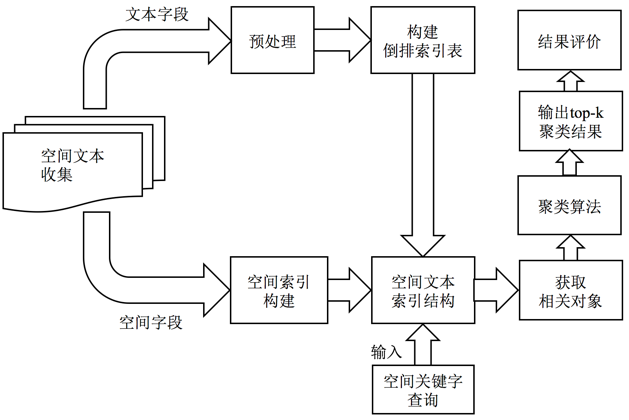
\includegraphics[width=5in]{process-of-design-topk.png}
		\caption{top-k空间文本簇检索设计流程}
		\label{topksearchprocess}
	\end{center}
\end{figure}

\subsection{top-k\ 空间文本簇查询定义}
\label{topk_definition}

定义一个数据集$D$,$p<\lambda,\varphi>\in D$,其中$p . \lambda$表示数据对象的位置信息,$p . \varphi$表示p的文本描述或文档信息(例如,餐馆的设施和菜单)。文档信息$p . \varphi$由一个向量$(w1, w2,...,wi)$表示,其中每个维度对应于文件中一个不同的词项$ti$。向量中每一项的权值$wi$用tf-idf值表示。词项$t$在文档$p$中出现的次数称为词项频率,记为$tf_{t,p}$。为了避免每个词项对于文档都同样重要(即对于文档的分类的贡献率相同),因此引入一个新的因子文档频率$df_{t}$,表示出现$t$的所有文档的数目。由于df本身往往较大,因此实际运用中需要映射到较小的取值上。为此,设定文档集总数为$N$,词项t的逆文档频率idf的定义如公式(\ref{idf})

\begin{equation}
	\label{idf}
	idf_{t} = log\frac{N}{df_{t}}
\end{equation}
对于一篇文档中的每个词项,将tf和idf组合形成最终的权重。tf-idf权重的最终计算公式如下:
\begin{equation}
	\label{tfidf}
	tfidf_{t,d} = tf_{t,d} \times idf_{t}
\end{equation}

\newpage

下面对于top-k空间文本簇给出相关扩展定义:

\begin{enumerate}[labelwidth=1.5cm,labelindent=10pt,leftmargin=2.2cm,label=\bfseries{ 定义 \arabic*:},align=left]
	\setcounter{enumi}{0}% just for the example
	
  \item 给定关键字集合\varphi和相关对象集合$D\varphi$,有(i) $D\varphi \in D$且(ii) $\forall p \in D\varphi$($\varphi \cap p. \varphi\neq\phi$).
  \item 有相关对象$p \in D_{\varphi}$,其$\varepsilon$-邻近点集合表示为$N\varepsilon(p)$,有$N\varepsilon(p) = { p_{i}\in D\varphi \mid \left| pp_{i}\right| < \varepsilon }$
  \item 相关对象$p$的$ \varepsilon $-邻近点集合$N \varepsilon (p)$如果是密集型的则表示该集合至少包含$minpts$个对象,即$\left| N \varepsilon (p) \right| \geq minpts$
  \item 如果相关对象$p$的$\varepsilon$-邻近点集合$N_{\varepsilon}(p)$是密集型的,则$p$为核心对象。
  \item 如果一组相关对象$p_{i}$ 和$p_{j}$是可直达的,则有: 
  \begin{enumerate}
		\item $p_{i} \in  N_{\varepsilon}(p_{j})$,且
		\item $\left| N_{\varepsilon}(p) \right| \geq minpts$
	\end{enumerate}
	
	\item 有一组可直达对象$p_{i}$和$p_{j}$以及一串相关对象$p_{1}, ..., p_{n}$,如果有$p_{i} = p_{1}, p_{j} = p_{n}$,则有$p_{m}和p_{m}+1$是可直达的,其中$1 \leq m < n.$ 

	\item 如果相关对象$p_{i}$和$p_{m}$可直达,相关对象$p_{j}$和$p_{m}$可直达,则称对象$p_{i}$和$p_{j}$可连接

	\item 一个空间文本聚类R同时满足: 
	\begin{enumerate}
		\item $R \subseteq D_{\varphi}$,且
		\item $R$是最大化集合,即当只考虑$D_{\varphi}$中的对象时,通过$\varepsilon$-邻近点集合$\forall p_{i},p_{j} \in R$满足$p_{i},p_{j}$是可连接的
	\end{enumerate}

\end{enumerate}

一个空间文本簇从数据集D中与关键词$\varphi$相关的对象集$D_{\varphi}$中找到的基于密度的簇。top-k空间文本簇(k-STC)查询$q =<\lambda, \varphi, k, \varepsilon, minpts>$有五个参数:$\lambda$表示点(用户)位置, $\varphi$表示一组关键词,$k$表示请求返回簇的数量,$\varepsilon$表示在邻近区域的距离约束,minpts表示密集型$\varepsilon$-邻域的密度阙值,即最少对象数量。k-STC将返回一个包含$k$个空间文本簇的列表,这些簇将由计分函数进行打分,并根据得分升序排列。基于密度的聚类算法使得每个簇都将最大化,意味着前$k$个簇不会重叠。密度约束参数$\varepsilon$, $minpts$依赖于用户的喜好,表明用户能够接受的移动范围。

直观地说,一个高文本相关性且位于查询位置附近的簇对应一个高排名的结果。簇$R$的计分函数如下:

\begin{equation}
	\label{evaluate}
	Scoreq(R) = \alpha\cdot d_{q.\lambda}(R)+(1-\alpha)\cdot (1-tr_{q.\varphi}(R))
\end{equation}

其中,$d_{q.\lambda}(R)$是查询位置$\lambda$与$R$中的对象之间的最小空间距离,本论文采用点在二维空间下欧式距离,即点$a = (x1, y1)$和$b = (x2, y2)$的距离为:

\begin{equation}
	\label{distance}
	d(a,b) = \sqrt{(x1-x2)^2 + (y1 - y2)^2};
\end{equation}

\newpage
$tr_{q.\varphi}(R)$是$R$中的最大文本相关性,$tr_(q.\psi)(R)=\sum_(t \in q.\psi \cap R.\psi)w_t $,相似度计算采用余弦相似度(cosine similarity),即对于文档$p1 = \vec{V}(p_1 ) = (w_1, w_2, ..., w_i), p_2 = \vec{V}(p_2) = (w_1, w_2, ..., w_i)$, 文档$p_1, p_2$的余弦相似度为:

\begin{equation}
	\label{simp1p2}
	sim(p_1, p_2) = \frac{\vec{V}(p_1) \cdot \vec{V}(p_2)}{\left| \vec{V}(p_1) \right| \cdot \left| \vec{V}(p_2) \right|} 
\end{equation}

分子为$\vec{V}(d_1)$和$\vec{V}(d_2)$的内积(inner product),分母为$\vec{V}(d_1)$和$\vec{V}(d_2)$的欧几里得长度的乘积。参数$\alpha$用于平衡簇的空间邻近性和文本相关性。


\subsection{top-k\ 空间文本簇检索系统架构}
本论文的空间文本簇检索系统架构按模块在大方向上分为数据处理模块和检索模块,数据处理模块又细分为分词模块、文本向量化模块、构建空间索引模块,分词模块调用了两个外部接口。分词模块和文本向量化模块将数据对象的文本信息转化为结构化信息,和由数据对象的空间信息构成的空间索引结构R-树一起构成空间文本索引结构IR-树。检索模块依据空间关键字在IR-树上查询邻域内相关对象,查找满足条件的簇。总体的系统架构图如图\ref{system_structure}所示:

\begin{figure}[htbp]
	% caption放上面就会显示在图的上方,出现在下面就是出现在图的下方
	% label的位置也有讲究
	\begin{center}
		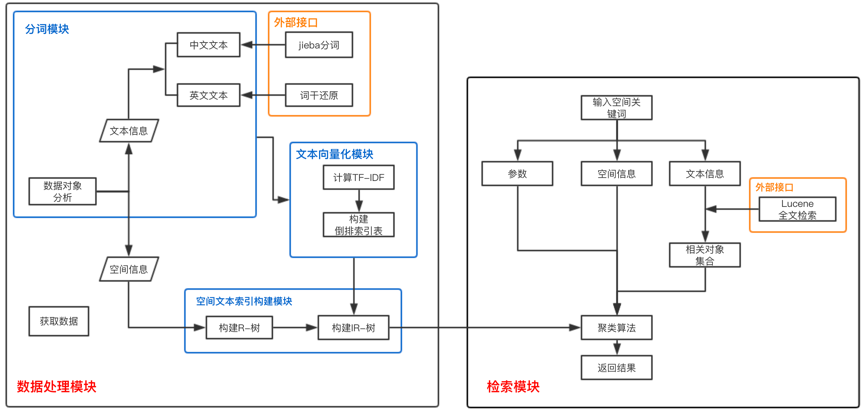
\includegraphics[width=6in]{structure-of-topk.png}
		\caption{top-k空间文本簇系统框架图}
		\label{system_structure}
	\end{center}
\end{figure}

\subsubsection{数据处理模块}

网络文本通常呈现出非结构化,不能被计算机直接处理。所以聚类首先需要将收集到的网络文本转换为结构化的数字信息,即空间文本表示模型。本论文采用向量空间模型(vector space model,简称VSM),向量空间模型是信息检索的基础,包括文档分类和聚类等,是目前数据挖掘中最常用的表示模型。另外常用的表示模型还有布尔模型和概率模型等。

数据处理模块通过文本分析将数据对象的文本描述信息传递给分词模块处理,分词模块根据中英文作出相应的分词处理;文本向量化模块则计算出分词后每个词项在文本中的权重,并构建倒排索引表。完成对单个文本的向量化处理后,构建向量空间模型,称为反向文件。最后将空间字段和反向文件传递给空间文本构建模块,建立IR-树。下面对每个小模块作进一步说明:

\textbf{1.分词模块:} 文本中,英文的表示以单词作为基本单位,单词之间以空格作为分隔符。根据分隔符划分文本并去除停用词后得到的词项结构已经可以达到了不错的分词效果。但是英文文本通常涉及到一个单词的多种形式,比如organize、organizes和organizing。还有表示相同意义的同源词,比如democracy、democratic和democratization。检索一个关键词时,对其同源词的检索会让结果更加有意义。而简单的利用标点和空格划分会使得单词的复现率高。词干(stem)还原[38]可以减少了单词的变化形式,或将派生词统一为基本形式。比如:

am, are, is => be

car, cars, car’s, cars’=> car

最常用的词干还原算法是Porter算法,算法复杂但是高效。值得注意的是,文本分词只是将自然语言结构化,词干还原方法使得检索更加全面但是并不会显著改善英文检索性能。

另一方面,对于中文分词,情况要复杂的多。中文没有直接的分隔符,灵活性和复杂性要比英文高得多。目前主要有三种中文分词方式:(1)基于统计的分词方法;(2)基于字符串匹配的分词方法(基于词典的方法);(3)基于理解的分词方法(基于规则的方法)。本研究将使用github上一种基于统计分词方法的开源中文分词项目jieba分词,对中文文本进行分词处理。 

分词模块将数据集的每一个文档按照文本字段和空间字段分别处理,文本字段即对象的描述内容,空间字段即对象的位置信息。分词模块会对分开处理中文文本和英文文本,对于中文文本,模块调用jieba分词接口进行分词处理,英文文本根据分隔符对单词进行预处理,再调用词干还原接口对单词作进一步处理。分词结果以词项列表的形式存储。通过接口处理完文本后,每个文本的词项都存储在内存中,并以传递给文本向量化模块。

\textbf{2.文本向量化模块:} 文本向量化模块根据每个文本的分词结果计算出每个词项的tf-idf值,以向量形式表示文本。首先,统计出一个词项词典d,该词典包含数据集D全部的词项t。然后,统计出每个词项对应tf和df值。根据公式(\ref{idf}) $idf_{t} = log\frac{N}{df_{t}}$和公式(\ref{tfidf})$tfidf_{t,d} = tf_{t,d} \times idf_{t}$ 计算出tf-idf值。至此,文档$p.\varphi$可以向量化表示为$(w_1, w_2,...,w_i),w_i=tf_i×idf_i$

文本检索中,我们需要根据关键词定位文档信息,所以我们需要一个从词项反向映射到文档的一种数据结构—反向文件。反向文件包含词项词典d,d中每一个词项都有一个记录包含该词项的所有文档的列表(称为倒排记录表,posting list),该表中的每一个元素表示词项在文档中的权重,即反向文件 = $\sum_{t_i \in d}(\sum_{p_i \cup t_i}(p_i,w_i))$。表\ref{reverse_file}为本论文所采用的反向文件的一个示例:

\begin{table}[h!]
  \begin{center}
    \caption{反向文件示例}
    \label{reverse_file}
    \begin{tabular}{l|l} % <-- Alignments: 1st column left, 2nd middle and 3rd right, with vertical lines in between
      \textbf{词典\ d} & \textbf{倒排索引表} \\
			\hline
			coffee & (p3, 0.5), (p6, 0.5), (p7, 0.5), (p1, 0.2), (p2, 0.2) \\
      tea & (p5, 0.5), (p7, 0.7), (p, 0.2), (p2, 0.3) \\
      pizza & (p4, 0.5)
    \end{tabular}
  \end{center}
\end{table}

\textbf{3.空间文本索引构建模块}的任务分为构建R树和构建IR树两个主要部分。R树是一种存储空间数据的树形数据结构,核心思想是将空间上距离相近的对象集合为一个节点并在其树结构中的父节点中将其表示为最小外接矩形(minimum bounding rectangle,MBR)。图\ref{rtree:example}展示了一个在二维空间上简单的R树的例子。p1-7为空间对象,Na,Nb,Nc,Nd为MBR。图\ref{rtree:mmb}展示了p1-7在空间上的而相对位置以及MBR的范围,MBR不断聚合最终形成图\ref{rtree:structure}所示的结构。 

\begin{figure}[htbp]
	\centering
	\begin{subfigure}{.5\textwidth}
		\centering
		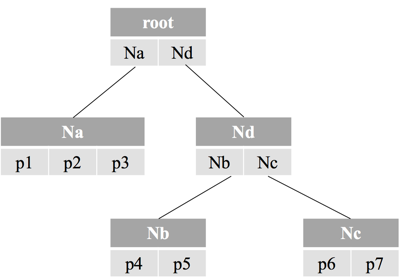
\includegraphics[width=.7\linewidth]{rtree-example.png}
		\caption{R树的数据结构}
		\label{rtree:structure}
	\end{subfigure}%
	\begin{subfigure}{.5\textwidth}
		\centering
		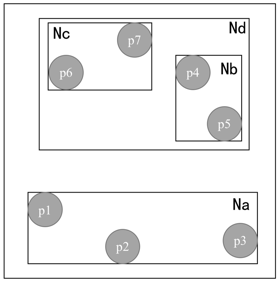
\includegraphics[width=.48\linewidth]{mbb-space-object.png}
		\caption{空间对象的MBB}
		\label{rtree:mmb}
	\end{subfigure}
	\caption{R树示例}
	\label{rtree:example}
\end{figure}

自底向上遍历R树,给每个节点创建反向文件。该反向文件记录了该节点下所有子节点或空间对象的倒排索引表。例如,定义空间对象的文本描述为$p=(w_1,w_2,…,w_i)$ ,假设$p4,p5$的文本描述为$p4 = ((pizza, 0.5)),p5 = ((tea, 0.5))$,则节点$Nb$的反向文件为$Nb = ((tea, p5), (pizza, p4))$。以表\ref{reverse_file}的反向文件为例,可以在图\ref{rtree:structure}的基础上得到如图\ref{ir_tree_example}所示的IR树,IR-树每个节点包含一个$e=(id,A,|D|)$形式的条目,其中$e.id$为节点标识符,$e. A$是对象空间位置的最小边界矩形, $e. \left| D \right|$是该节点内空间对象或子节点的数量。每个节点还包含一个指向反向文件的指针。非叶子同叶子节点有相同的条目,但其子节点为非叶子或叶子节点,不直接包含空间对象。

\begin{figure}[htbp]
	% caption放上面就会显示在图的上方,出现在下面就是出现在图的下方
	% label的位置也有讲究
	\begin{center}
		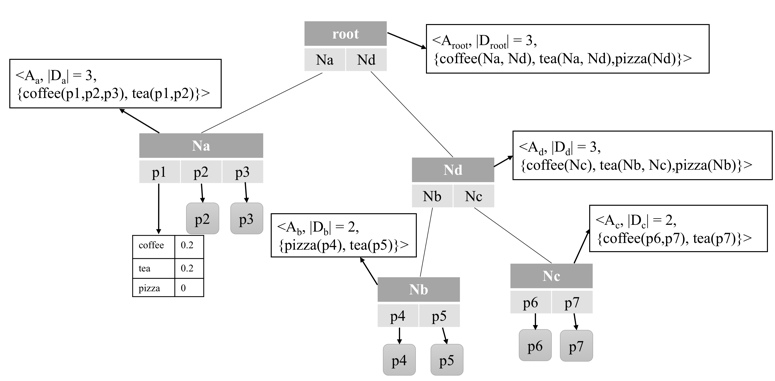
\includegraphics[width=5in]{ir-tree.png}
		\caption{top-k空间文本簇系统框架图)}
		\label{ir_tree_example}
	\end{center}
\end{figure}
\subsubsection{查询模块}

由\ref{topk_definition}节可知,top-k空间文本簇(k-STC)查询$q=<\lambda, \varphi, k, \varepsilon, minpts>$有五个参数,\textbf{查询模块}会将参数分为3个字段,一个是文本字段,即一组关键词$\varphi$;一个是空间字段,即查询位置$\lambda$;最后一个是调节参数,包含距离约束$\varepsilon$,密度阙值$minpts$,请求簇的数量$k$。
通过全文检索系统Lucene检索文档集,返回包含关键词的文档集$D_\varphi$。选取一个文档作为核心对象执行聚类算法,找到以该核心对象为中心的簇,如果有满足参数条件$(\varepsilon,minpts)$的簇则计算簇得分(公式\ref{simp1p2}),加入候选列表。最终返回$k$个得分较好的簇。

\subsection{top-k空间文本簇查询处理算法}

聚类算法选择基于密度的聚类方法中最具代表性的DBSCAN算法。DBSCAN随机选取一个对象作为核心点,检查核心点的邻近领域是否至少有若干个对象,满足则对邻近对象继续迭代检查,不满足而标记噪点。邻近区域的大小和密度阙值由用户决定。

DBSCAN算法的一个基本方案是,给定一个查询,根据查询关键字获得相关的对象集$D\varphi$,然后找到所有满足密度约束的簇,根据得分函数(公式\ref{simp1p2})排序,返回最优的$k$个簇。但是这个方案效率很低,因为查找所有簇的开销很大。研究[3]提出了一种BASIC算法,该算法能够在不查找所有簇的情况下返回最顶层的$k$个簇。BASIC算法将前期得到的集群作为候选集群,然后根据第$k$个候选集群的得分设置阈值。BASIC算法对所有未来将找到的集群分数估计一个边界值,如果边界值比阈值低,则当前候选集群为最终结果。BASIC算法的提前停止条件大大提高了聚类效率。

\begin{algorithm}
	\caption{BASIC}
	\label{basic_alg}
	\begin{algorithmic}[1] %每行显示行号
			\Require 查询关键词$ q=<λ,φ,k,ε,minpts>$, IR-树 $irtree$, 反向文件索引 $iindex$
			\Ensure $rlist$

			\State $D_\psi \gets (q.\varpsi,iindex)$ \qquad(获取与查询关键字相关的对象)

			\State $slist \gets$ 将$D_\psi$中的对象按照$dq.\lambda(p.\lambda)$升序排列;
			\State $tlist \gets$ 将$D_\psi$中的对象按照$1-tr_{q.\psi} (p.\psi)$升序排列;
			
			\State $rlist \gets \phi$ // $rlist$保存候选集群,初始化为空;

			\State $\tau \gets \infty$ //阙值初始为无限大;
			
			\Repeat 

			\State 对象$ \gets (slist, tlist)$

			\State c $\gets \textbf{GetCluster}(p,q,irtree,tlist,slist)$ 
			
			\If {$c \neq \phi$}
				\State 将$c$加入$rlist$;

				\State $\tau $更新为$rlist$第$k$个集群的得分(公式\ref{evaluate});

				\State $sb \gets slist$的首元素;

				\State $tb \gets tlist$的首元素;

				\State $bound \gets \alpha · sb+(1-\alpha)·tb;$ // 设定边界值
			\EndIf

			\Until{$bound \geq \tau ∨ slist=\phi$} 
			
		\State \Return{rlist}
	\end{algorithmic}
\end{algorithm}

算法\ref{basic_alg}为BASIC算法的伪代码。它首先获得相关的对象集$D$ (第1行);其次,根据$D$中对象到查询点的距离降序排列,得到$slist$ (第2行);根据$D$中对象和查询关键字的相关程度排序(第3行)。候选列表$rlist$初始化为空(第4行);阈值设置为无穷大(第5行)。同时按书按需遍历slist和tlist 的元素(第7行);执行GetCluster方法(算法\ref{getcluster}),尝试查找包含以p为核心对象的簇(第8行),如果找到满足条件的簇,将其添加到$rlist$并更新阙值(9 - 11行)。计算待检查集群的边界值(12 - 14行)。当边界值大于阙值或$slist$为空(那么$tlist$也为空)(15行)。最终确定了$rlist$中的前k个候选集群。

\begin{algorithm}
	\caption{GetCLuster}
	\label{getcluster}
	\begin{algorithmic}[1] %每行显示行号
			\Require 核心对象 $p$, 查询关键词$q=<\lambda,\varphi,k,\varepsilon, minpts>$, IR-树 $irtree,List slist, List tlist$
			\Ensure 集群$R$

			\State $R \gets \phi$

			\State $neighbors \gets RangeQuery(itree, q, p)$ // 获取p的邻近对象

			\If {$neighbors.size < q.minpts $}

				\State 将p从slist,tlist中移除;

				\State 将p标记为噪点;

				\State \Return{R}
			\Else
				\State 将$neighbors$的对象加入$R$且从$slist$,$tlist$中移除;
				\For{\textbf{each}$ p_i \in neighbors$}
				
						\State $neighborsi \gets RangeQuery(irtree,q,p_i);$
						\If{neighborsi.size ≥ q.minpts}
							\For{\textbf{each} $p_j \in neighbors_i$}
								\If{$p_j$ 是噪点} 
										\State 将$p_j$加入$R$;
								\ElsIf{$p_j \notin R$}
									\State 将$p_j$加入$R$,并将$p_j$移除$slist$,$tlist$;
									\State 将$p_j$加入$neighbors$;
								\EndIf
							\EndFor
						\EndIf
				\EndFor
			\EndIf

	\State \Return{R}
	\end{algorithmic}
\end{algorithm}


算法\ref{getcluster}是检索以$p$为核心对象的密集邻域簇R的方法GetCluster的伪代码。执行方法RangeQuery(算法\ref{rangequery}),在半径为ε的领域内查找相关对象(第2行)。如果其领域范围内的对象数小于$q.minpts$,对象$p$被标记为噪音,并返回一个空集(第3-6行)。否则,其邻域的点加入簇R(第8行)。然后,查找以该邻域内的对象为核心的簇并判断是否密集(第9-10行)。如果是密集邻域,将邻域内先前标记为噪声或未加入簇R的对象添加到簇$R$中(第13-
16行)。但簇R的对象不能再增加时,返回簇$R$。

\begin{algorithm}
	\caption{RangeQuery}
	\label{rangequery}
	\begin{algorithmic}[1] %每行显示行号
			\Require $p$查询关键词$q=<\lambda,\varphi,k,\varepsilon, minpts>$, IR-树 $irtree$
			\Ensure 邻近节点集合$neighbors$

			\State $neighbors \gets \phi$

			\State $queue \gets \phi$ // $queue$为队列
			
			\State $queue.Enqueue( irtree.root);$

			\While{$queue \neq null$}

				\State $e \gets queue.Dequeue();$

				\State $N \gets ReadNode(e); $// 读取节点e并赋值给N

					 \If{$N$是叶子节点}
					 
							 \For{\textbf{each} $o \in N$}
							 
									\If {$o$ 是$q$的相关对象且$\left|p o \right|_min min \leq 
									 q.\varepsilon$}
											\State  $neighours.Add(o);$
									\EndIf
								\EndFor
						\Else

							\For{\textbf{each} $\left|e'o \right|_min min \leq q.\varepsilon$}

								\If{$e'$和$q$相关且$\left|e' o|min \leq q.\varepsilon$}

									\State $queue.Enqueue(e');$

								\EndIf
							
							\EndFor
							
						\EndIf
			
						
			\EndWhile
		\State \Return{$neighbors$}
	\end{algorithmic}
\end{algorithm}

算法\ref{rangequery}是查找对象邻域的方法RangeQuery的伪代码。RangeQueue通过IR树找到慢满足约束的对象。首先,将IR-tree的根节点添加到队列中。循环访问队列节点。如果是叶子节点,对于其包含的满足距离约束的相关的对象,加入到邻居集合。如果该节点是非叶节点。它的子节点与查询关键字相关,并且位于邻域范围,则将该节点加入到优先队列。当队列为空时,返回邻居集合。

\subsection{top-k空间文本簇查询处理算法优化}

从BASIC算法可知,越早找到得分更好(更小)的簇将越早结束计算。集群的得分由两部分组成,集群到查询点的距离越近,文本相似度越高,簇分数越好。算法\ref{basic_alg}的2-3行就是从这两个方面,分别针对对于查询点来说距离越近,相似度越高的邻近节点进行集群检测。那么,可以设想,如果将对查询点的有序检测推广到每一次集群检测中,将从更小的范围提前找到优秀的邻近节点。

例如,将图\ref{ir_tree_example}中节点的倒排索引表展开,可以得到如图\ref{ir_tree_structure_ig_node_rev_file}所示的结构。

\begin{figure}[htbp]
	% caption放上面就会显示在图的上方,出现在下面就是出现在图的下方
	% label的位置也有讲究
	\begin{center}
		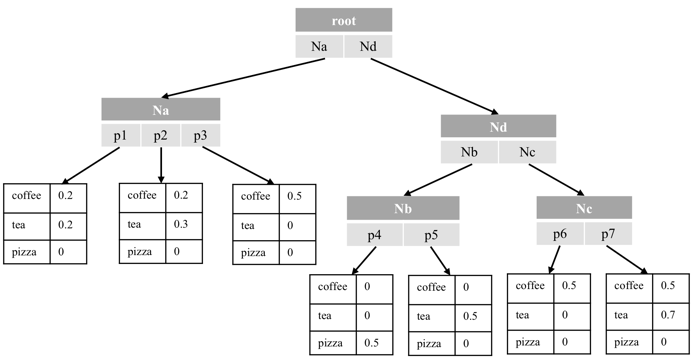
\includegraphics[width=5in]{ir-tree-ignore-nodereverse.png}
		\caption{IR-树结构图(省略节点的反向文件)}
		\label{ir_tree_structure_ig_node_rev_file}
	\end{center}
\end{figure}

当检索“tea”时,假设每个节点与查询点的距离满足约束条件,检查节点的顺序为层次遍历,那么可得遍历的顺序为($p1,p2,p5,p$7),假设不在同一个叶子节点内的对象间不能都成集群(距离约束),集群至少有一个对象,返回1个集群结果。那么可以得到$rlist$的变化过程,如表\ref{cluster_table}所示,总共需要进行4次临界值比较和4次得分计算,当有N个相关对象时,最坏情况下需要计算N次。

\begin{table}[h!]
  \begin{center}
    \caption{反向文件示例}
    \label{cluster_table} 
    \begin{tabular}{l|l|l} % <-- Alignments: 1st column left, 2nd middle and 3rd right, with vertical lines in between
      \textbf{次数\ d} & \textbf{候选集群} & \textbf{淘汰集群} \\
			\hline
			0 & \{\}& \{\} \\
			1 & \{c(p1)\} & \{\} \\
			2 & \{c(p2)\} & \{c(p1)\} \\
			3 & \{c(p3)\} & \{c(p1), c(p2)\} \\
			4 & \{c(p4)\} & \{c(p1, c(p2), c(p5))\} \\
    \end{tabular}
  \end{center}
\end{table}

由图\ref{ir_tree_structure_ig_node_rev_file}可知,当检索“tea”时,最佳的检索书顺序是($p7,p5,p2,p$1),这种情况下将进行4次临界值比较和1次得分计算,当有N个相关对象时,最坏情况下需要计算k次。通常情况下,k 远远小于N。

\begin{figure}[htbp]
	% caption放上面就会显示在图的上方,出现在下面就是出现在图的下方
	% label的位置也有讲究
	\begin{center}
		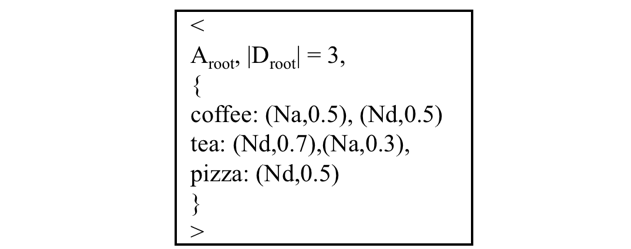
\includegraphics[width=4in]{root-reverse-file.png}
		\caption{根节点反向文件}
		\label{root_reverse_file}
	\end{center}
\end{figure}